\documentclass[conference]{IEEEtran}
\IEEEoverridecommandlockouts
\usepackage{cite}
\usepackage{amsmath,amssymb,amsfonts}
\usepackage{algorithmic}
\usepackage{graphicx}
\usepackage{textcomp}
\usepackage{xcolor}
\usepackage{booktabs}
\usepackage{url}
\usepackage{multirow}

\def\BibTeX{{\rm B\kern-.05em{\sc i\kern-.025em b}\kern-.08em
    T\kern-.1667em\lower.7ex\hbox{E}\kern-.125emX}}

\begin{document}

\title{On-Device Acoustic Gunshot Detection: Data Cleaning, Model Comparison, and a One-Bit Edge Alert}

\author{
\IEEEauthorblockN{1\textsuperscript{st} Jeevant Sharma}
\IEEEauthorblockA{\textit{Department of Computer Science and Engineering} \\
\textit{Indian Institute of Information Technology, Surat}\\
Surat, India \\
jeevant.sharma@iiitsurat.ac.in}
\and
\IEEEauthorblockN{2\textsuperscript{nd} Deepesh Dangi}
\IEEEauthorblockA{\textit{Department of Computer Science and Engineering} \\
\textit{Indian Institute of Information Technology, Surat}\\
Surat, India \\
deepesh.dangi@iiitsurat.ac.in}
\and
\IEEEauthorblockN{3\textsuperscript{rd} Dr. Kaustubh Dhondge}
\IEEEauthorblockA{\textit{Department of Computer Science and Engineering} \\
\textit{Indian Institute of Information Technology, Surat}\\
Surat, India \\
kaustubh@iiitsurat.ac.in}
}

\maketitle

% ==============================================================================
% ABSTRACT
% ==============================================================================
\begin{abstract}
Acoustic gunshot detection on low-cost embedded edge platforms presents physical challenges including transducer domain shift, diaphragm saturation at high sound pressure levels, electrical DC voltage rail drift, thermal ADC hiss amplification, and false triggers from percussive imposter sounds. This paper reports a detector designed for deployment on an Arduino Nano 33 BLE Sense. Training and evaluation were conducted on a host PC. Edge timing was profiled on a virtual machine throttled to 45--50\% CPU utilization to approximate a Raspberry Pi~4. Audio data was cleaned using librosa at window lengths of 250\,ms, 500\,ms, and 1\,s. The operational window is 750\,ms, since a 250\,ms cut removes the reverberation decay that distinguishes a gunshot from a percussive knock. Classical classifiers (logistic regression, SVM, random forest) achieved 99--100\% accuracy on balanced hold-out files but failed on live microphone input. Five neural architectures were trained and evaluated. On a 1{,}442-clip balanced hold-out, three models exceed 99.5\% accuracy. On 300 unseen recordings, the best single-model sliding-window gunshot recall is 67\%, achieved by the Enhanced 2D CNN which executes in 0.09\,ms within a 123.6\,KB INT8 footprint. A three-model ensemble raises recall to 77\% within 715\,KB and 17\,ms combined. The PCEN-based CRNN exhibits zero recall degradation under simulated microphone distortion, confirming Per-Channel Energy Normalization as an effective domain-shift normalizer for heterogeneous edge hardware. The proposed deployment architecture retains all audio on the sensor node, transmits only a single-bit detection flag (1~for gunshot, silence otherwise), and requires spatial consensus from multiple neighbouring nodes at the gateway before raising an alert.
\end{abstract}

\begin{IEEEkeywords}
Acoustic gunshot detection, edge inference, TinyML, PCEN, convolutional recurrent neural networks, Arduino Nano 33 BLE Sense, one-bit transmission.
\end{IEEEkeywords}

% ==============================================================================
% SECTION I: INTRODUCTION
% ==============================================================================
\section{Introduction}
\label{sec:intro}

Firearm violence in urban and peri-urban environments demands rapid, automated detection and localization of gunshot events. Empirical studies indicate that a significant fraction of firearm discharges in affected neighbourhoods are never reported by witnesses. When reports are made, they are frequently delayed and spatially inaccurate. An automated acoustic sensing system deployed across a campus, urban block, or wildlife sanctuary can detect the event within seconds and dispatch emergency response to the precise location. The same listening problem extends to forests and national sanctuaries, where gunshots and illegal logging threaten wildlife.

Dense urban environments present the hardest deployment scenario due to continuous traffic, construction, and festival fireworks. Institutional campuses---colleges, schools, government perimeters---offer a more controlled starting point with known site geometry and reduced ambient impulsive noise. Even with existing technological infrastructure, adoption remains uneven: in regions with dense populations and limited resources, autonomous acoustic monitoring within institutional boundaries represents a practical first deployment.

An authentic acoustic gunshot discharge consists of two physical phenomena:
\begin{enumerate}
    \item A supersonic projectile shockwave (N-wave), characterized by an abrupt non-linear pressure rise lasting $1\,\text{ms}$ to $5\,\text{ms}$.
    \item An explosive muzzle blast accompanied by an environmental reverberation decay tail spanning $200\,\text{ms}$ to $600\,\text{ms}$.
\end{enumerate}

The target deployment platform is the Arduino Nano 33 BLE Sense (nRF52840, Cortex-M4F, 1\,MB Flash, 256\,KB SRAM). The node must execute inference locally without streaming microphone audio to any external server, preserving civilian privacy. This paper covers the stages preceding physical deployment: model training on a PC, conversion from Keras (\texttt{.h5}) to TensorFlow Lite (\texttt{.tflite}), INT8 quantization, and latency profiling on a virtual Raspberry Pi. The deployment design---duty-cycled sleep, one-bit radio transmission, and multi-node spatial consensus at a gateway---is described in Section~\ref{sec:conclusion}.

The remainder of this paper is organized as follows. Section~\ref{sec:related} reviews related work. Section~\ref{sec:data} describes the data pipeline and preprocessing. Section~\ref{sec:conditioning} addresses hardware conditioning for edge deployment. Section~\ref{sec:models} details the model architectures. Section~\ref{sec:setup} defines evaluation protocols. Section~\ref{sec:results} presents experimental results. Section~\ref{sec:conclusion} discusses conclusions and planned hardware deployment.

% ==============================================================================
% SECTION II: RELATED WORK
% ==============================================================================
\section{Related Work}
\label{sec:related}

Municipal acoustic surveillance systems have demonstrated the viability of city-scale gunshot detection. Open datasets such as the multi-firearm, multi-orientation recording set published in \emph{Data in Brief}~\cite{dib2023} provide calibrated multi-caliber recordings for research use. Commercial systems validate the concept but typically require continuous audio streaming to centralized cloud infrastructure, raising bandwidth costs and civilian privacy concerns that are incompatible with campus-scale edge deployment.

Per-channel energy normalization (PCEN) was proposed for bioacoustic sound event detection~\cite{lostanlen2019}. PCEN divides each frequency band by a smoothed running estimate of its own background energy, suppressing stationary noise (rain, wind, HVAC hum) while preserving sudden transient impulses. One of our models adopts this front-end. The network architecture, training data, and evaluation methodology presented in this paper are original to this work.

Edge Impulse~\cite{edgeimpulse2024} was used as a preliminary TinyML evaluation platform on an ARM Cortex-M4F target prior to our main TensorFlow-based models. MixUp regularization~\cite{zhang2018} and SpecAugment~\cite{park2019} are employed within the enhanced convolutional architectures. CNN-based large-scale audio classification~\cite{hershey2017} and forest acoustic monitoring~\cite{saha2025} provide additional architectural context for spectrogram-domain approaches.

% ==============================================================================
% SECTION III: DATA PIPELINE AND PREPROCESSING
% ==============================================================================
\section{Data Pipeline and Preprocessing}
\label{sec:data}

\subsection{Audio Ingestion and Data Volume}
The raw data pool comprised approximately 80{,}000 audio files aggregated from multiple sources:
\begin{itemize}
    \item \textbf{Calibrated Gunshot Dataset}: Multi-firearm, multi-orientation recordings from Data in Brief~\cite{dib2023}, featuring calibrated multi-caliber and multi-angle recordings.
    \item \textbf{Raw Firearm Files}: 4{,}138 recordings encompassing handguns, rifles, and shotguns across open-field and indoor acoustic geometries.
    \item \textbf{Ambient Repositories}: 6{,}230 long-duration source recordings (10\,s to 60\,min) containing urban traffic, rainfall, construction, human speech, and room acoustics.
\end{itemize}
Cleaning was performed using librosa. Approximately 1{,}000 to 5{,}000 clips were manually audited in iterative listening cycles until the retained clips met quality requirements.

\subsection{Window Length Selection}
Candidate window lengths of 250\,ms, 500\,ms, and 1\,s were evaluated. The muzzle blast attack lasts only a few milliseconds, but the environmental reverberation decay persists for several hundred milliseconds. A 250\,ms window retains the attack but discards most of the decay, causing gunshots and percussive knocks to become spectrally similar. The operational window was set to \textbf{750\,ms} (16{,}537 samples at 22{,}050\,Hz). On the live inference path, consecutive windows overlap by 75\% (hop of 187.5\,ms) to ensure that any transient event falls fully within at least one analysis frame.

\subsection{Onset Detection and Quality Gates}
Audio segmentation uses a 3-way candidate onset detector:
\begin{enumerate}
    \item \textbf{Spectral Flux}: Computes positive frame-to-frame spectral energy surges via half-wave rectification across STFT bins:
    \begin{equation}
        O(m) = \sum_{k} \max\left(0, |X(k, m)| - |X(k, m\!-\!1)|\right)
        \label{eq:spectral_flux}
    \end{equation}
    where $X(k, m)$ denotes the STFT magnitude at frequency bin $k$ and frame $m$.
    \item \textbf{Raw Amplitude Peak}: Indexes the maximum absolute sample $n_{\text{peak}} = \arg\max_n |y[n]|$.
    \item \textbf{Smoothed Discrete Envelope}: Convolves the absolute signal with a moving-average kernel ($K = 0.005 \cdot f_s$) to filter single-sample electrical spikes.
\end{enumerate}

Every extracted candidate is evaluated against three physical quality gates to prevent label contamination:
\begin{equation}
    \text{Crest Factor} = \frac{\max(|y|)}{\text{RMS} + \epsilon}
    \label{eq:crest_factor}
\end{equation}
\begin{equation}
    \text{Prominence} = \frac{\max(|y|)}{\text{Median}(|y|) + \epsilon}
    \label{eq:prominence}
\end{equation}
\begin{equation}
    \text{Attack Ratio} = \frac{\sum_{n=0}^{N/2-1} y[n]^2}{\sum_{n=N/2}^{N-1} y[n]^2 + \epsilon}
    \label{eq:attack_ratio}
\end{equation}
Negative-class slices exhibiting high attack ratios combined with extreme crest factors are purged, ensuring the negative training corpus remains free of percussive transients.

\subsection{Class Balance}
Initial 1:1 gunshot-to-non-gunshot ratios produced the 99--100\% classical accuracy figures. Continuous monitoring approximates 1:10 to 1:50 ratios, since almost every window is silence, speech, or traffic. Later training used negative-heavy ratios to prevent overconfident predictions on ordinary sounds.

% ==============================================================================
% SECTION IV: HARDWARE CONDITIONING
% ==============================================================================
\section{Hardware Conditioning for Edge Deployment}
\label{sec:conditioning}

Transitioning neural models from laboratory WAV files to embedded micro-sensors (electret capsules and I2S MEMS INMP441 transducers on Raspberry Pi) exposes three hardware-level distortions. Fig.~\ref{fig:pipeline} illustrates the complete edge conditioning pipeline.

\begin{figure}[!t]
\centering
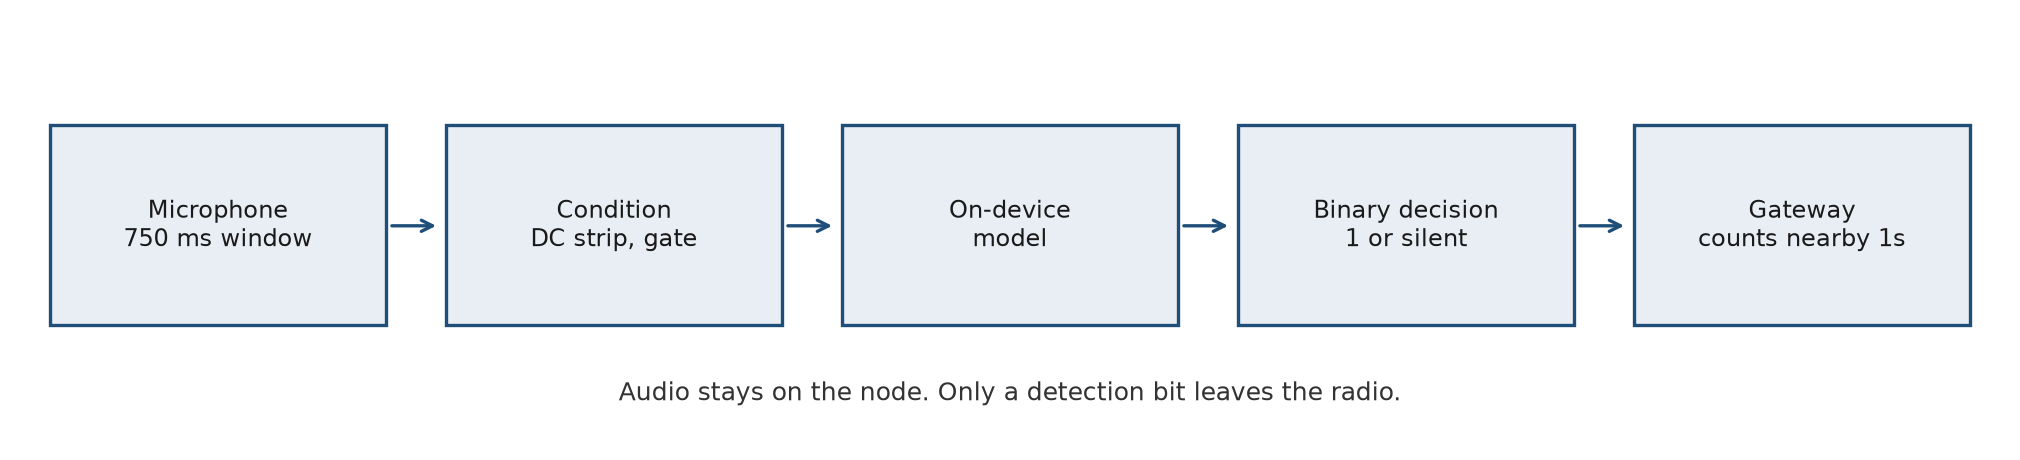
\includegraphics[width=\columnwidth]{figures/fig1_edge_pipeline.png}
\caption{Edge inference pipeline. A circular ring buffer enforces 750\,ms framing with 75\% hop overlap. DC offset stripping, energy-gated normalization, and INT8 quantized inference execute on-device. Only a detection bit reaches the gateway.}
\label{fig:pipeline}
\end{figure}

\subsection{DC Voltage Rail Drift}
Low-cost sensors on 3.3\,V or 5.0\,V supply rails exhibit resting baseline drift ($+0.05$ to $-0.08$\,V) from supply ripple and uncalibrated preamplifiers. This phantom DC energy skews convolutional activation distributions. The preconditioning stage removes the offset:
\begin{equation}
    y_{\text{clean}}[n] = y[n] - \frac{1}{N}\sum_{i=0}^{N-1} y[i]
    \label{eq:dc_strip}
\end{equation}

\subsection{Thermal ADC Hiss and Energy-Gated Normalization}
Standard peak normalization ($y / \max(|y|)$) produces catastrophic failure in quiet conditions. When peak amplitude $\approx 0.002$, normalization amplifies thermal ADC noise by up to $500\times$. An energy gate prevents this:
\begin{equation}
    y_{\text{cond}} = 
    \begin{cases} 
        y / \max(|y|) & \text{if } \text{RMS} \ge 0.005 \\
        y & \text{if } \text{RMS} < 0.005
    \end{cases}
    \label{eq:energy_gate}
\end{equation}

\subsection{Diaphragm Saturation}
A firearm discharge at close proximity exceeds $120\,\text{dB}$ SPL, saturating consumer micro-sensor diaphragms into square-wave clipping. Hard-clipping and non-linear dynamic range compression are incorporated into training augmentation to build resilience against saturated waveforms.

% ==============================================================================
% SECTION V: MODEL ARCHITECTURES
% ==============================================================================
\section{Model Architectures}
\label{sec:models}

Five neural models share the 750\,ms conditioning front-end described in Section~\ref{sec:conditioning}. Table~\ref{tab:models} summarizes the architectures.

\begin{table}[!t]
\centering
\caption{Neural model specifications.}
\label{tab:models}
\footnotesize
\begin{tabular}{lrrl}
\toprule
\textbf{Model} & \textbf{Params} & \textbf{INT8} & \textbf{Edge Status} \\
\midrule
Baseline 1D CNN & 92{,}513 & 112.5\,KB & Compatible \\
Baseline 2D CNN & 249{,}985 & 259.9\,KB & Compatible \\
Enhanced 1D CNN & 96{,}674 & 118.5\,KB & Quant. Failure \\
Enhanced 2D CNN & 110{,}594 & 123.6\,KB & \textbf{Top (0.09\,ms)} \\
CRNN-PCEN & 397{,}842 & 478.9\,KB & Robust (11.86\,ms) \\
\bottomrule
\end{tabular}
\end{table}

\subsection{Baseline 1D Raw-Waveform CNN (92{,}513 Parameters)}
This model operates directly on 16{,}537 raw audio samples, bypassing spectral transformation entirely. Table~\ref{tab:arch_1d} details the layer-by-layer topology.

\begin{table}[!t]
\centering
\caption{Baseline 1D CNN architecture (\texttt{1D\_CNN\_GunShot\_Detector}).}
\label{tab:arch_1d}
\footnotesize
\begin{tabular}{llcc}
\toprule
\textbf{Layer} & \textbf{Config} & \textbf{Output Shape} & \textbf{Params} \\
\midrule
Input & --- & $(16537, 1)$ & 0 \\
Conv1D & $K\!=\!80$, $S\!=\!4$, 32 & $(4135, 32)$ & 2{,}592 \\
BatchNorm & --- & $(4135, 32)$ & 128 \\
MaxPool1D & $P\!=\!4$ & $(1033, 32)$ & 0 \\
Conv1D & $K\!=\!3$, 64 & $(1033, 64)$ & 6{,}208 \\
BatchNorm & --- & $(1033, 64)$ & 256 \\
MaxPool1D & $P\!=\!4$ & $(258, 64)$ & 0 \\
Conv1D & $K\!=\!3$, 128 & $(258, 128)$ & 24{,}704 \\
BatchNorm & --- & $(258, 128)$ & 512 \\
Conv1D & $K\!=\!3$, 128 & $(258, 128)$ & 49{,}280 \\
BatchNorm & --- & $(258, 128)$ & 512 \\
GlobalAvgPool1D & --- & $(128)$ & 0 \\
Dense & 64, ReLU & $(64)$ & 8{,}256 \\
Dropout & 0.4 & $(64)$ & 0 \\
Dense & 1, Sigmoid & $(1)$ & 65 \\
\bottomrule
\end{tabular}
\end{table}

The first convolutional layer uses an 80-sample kernel. At $f_s = 22{,}050\,\text{Hz}$, this spans:
\begin{equation}
    \Delta t = \frac{80}{22{,}050} \approx 3.63\,\text{ms}
    \label{eq:kernel_duration}
\end{equation}
This layer functions as a learnable bank of 32~finite impulse response (FIR) filters, each wide enough to capture the full rise-time of a supersonic N-wave shockwave. The stride of 4 provides $4\times$ temporal downsampling while preserving transient onset positions. Subsequent $K\!=\!3$ convolutions with BatchNormalization refine local acoustic patterns. Max-pooling is applied only after the first two convolutional blocks to preserve temporal resolution during the rapid attack--decay transition. Global Average Pooling compresses 258 time steps into a single 128-dimensional feature vector before the classification head, providing superior generalization compared to flattening.

\subsection{Baseline 2D Mel-Spectrogram CNN (249{,}985 Parameters)}
This model transforms raw audio into a 2D time-frequency representation: a 64-band log-mel spectrogram over 130~time frames ($N_{\text{fft}} = 512$, hop $H = 128$). Table~\ref{tab:arch_2d} details the architecture.

\begin{table}[!t]
\centering
\caption{Baseline 2D CNN architecture (\texttt{2D\_CNN\_LogMel}).}
\label{tab:arch_2d}
\footnotesize
\begin{tabular}{llcc}
\toprule
\textbf{Layer} & \textbf{Config} & \textbf{Output Shape} & \textbf{Params} \\
\midrule
Input & --- & $(64, 130, 1)$ & 0 \\
Conv2D & $(3\!\times\!3)$, 32 & $(64, 130, 32)$ & 320 \\
BatchNorm & --- & $(64, 130, 32)$ & 128 \\
MaxPool2D & $(2\!\times\!2)$ & $(32, 65, 32)$ & 0 \\
Conv2D & $(3\!\times\!3)$, 64 & $(32, 65, 64)$ & 18{,}496 \\
BatchNorm & --- & $(32, 65, 64)$ & 256 \\
MaxPool2D & $(2\!\times\!2)$ & $(16, 32, 64)$ & 0 \\
Conv2D & $(3\!\times\!3)$, 128 & $(16, 32, 128)$ & 73{,}856 \\
BatchNorm & --- & $(16, 32, 128)$ & 512 \\
Conv2D & $(3\!\times\!3)$, 128 & $(16, 32, 128)$ & 147{,}584 \\
BatchNorm & --- & $(16, 32, 128)$ & 512 \\
GlobalAvgPool2D & --- & $(128)$ & 0 \\
Dense & 64, ReLU & $(64)$ & 8{,}256 \\
Dropout & 0.4 & $(64)$ & 0 \\
Dense & 1, Sigmoid & $(1)$ & 65 \\
\bottomrule
\end{tabular}
\end{table}

Max-pooling is restricted to the first two convolutional blocks. Blocks 3 and 4 omit pooling to preserve temporal resolution during the rapid attack--decay transition of gunshot spectrograms. The 2D convolutions learn joint time-frequency patterns that 1D models cannot capture from raw waveforms.

\textit{Dying ReLU Collapse}: An early training run fed unnormalized decibel values ($-80$ to $0$\,dB) into ReLU activations. Since ReLU outputs zero for all negative inputs, the entire input range produced zero activations, extinguishing all gradients and yielding 0\% recall (721 false negatives). Rescaling inputs to $[0,1]$:
\begin{equation}
    S_{\text{norm}} = \frac{S_{\text{dB}} + 80}{80}
    \label{eq:norm_db}
\end{equation}
restored convergence to 99.86\% ROC-AUC.

\subsection{Enhanced Dual-Head Models}
The Enhanced variants extend the baseline architectures with a shared backbone that branches into two classification heads after Global Average Pooling. Table~\ref{tab:arch_enh2d} shows the Enhanced 2D CNN (primary production model). The Enhanced 1D CNN shares the same 1D backbone with a dual-head split.

\begin{table}[!t]
\centering
\caption{Enhanced 2D CNN architecture (\texttt{Enhanced\_2D\_CNN\_DualHead}).}
\label{tab:arch_enh2d}
\footnotesize
\begin{tabular}{llcc}
\toprule
\textbf{Layer} & \textbf{Config} & \textbf{Output Shape} & \textbf{Params} \\
\midrule
Input & --- & $(64, 33, 1)$ & 0 \\
Conv2D & $(3\!\times\!3)$, 16 & $(64, 33, 16)$ & 160 \\
BatchNorm & --- & $(64, 33, 16)$ & 64 \\
MaxPool2D & $(2\!\times\!2)$ & $(32, 16, 16)$ & 0 \\
Conv2D & $(3\!\times\!3)$, 32 & $(32, 16, 32)$ & 4{,}640 \\
BatchNorm & --- & $(32, 16, 32)$ & 128 \\
MaxPool2D & $(2\!\times\!2)$ & $(16, 8, 32)$ & 0 \\
Conv2D & $(3\!\times\!3)$, 64 & $(16, 8, 64)$ & 18{,}496 \\
BatchNorm & --- & $(16, 8, 64)$ & 256 \\
MaxPool2D & $(2\!\times\!2)$ & $(8, 4, 64)$ & 0 \\
Conv2D & $(3\!\times\!3)$, 128 & $(8, 4, 128)$ & 73{,}856 \\
BatchNorm & --- & $(8, 4, 128)$ & 512 \\
GlobalAvgPool2D & --- & $(128)$ & 0 \\
\midrule
\multicolumn{4}{l}{\textit{Head 1: Gunshot Detection}} \\
Dense & 64, ReLU & $(64)$ & 8{,}256 \\
Dropout & 0.4 & $(64)$ & 0 \\
Dense & 1, Sigmoid & $(1)$ & 65 \\
\midrule
\multicolumn{4}{l}{\textit{Head 2: Anomaly Score}} \\
Dense & 32, ReLU & $(32)$ & 4{,}128 \\
Dropout & 0.3 & $(32)$ & 0 \\
Dense & 1, Sigmoid & $(1)$ & 33 \\
\bottomrule
\end{tabular}
\end{table}

The Enhanced architecture incorporates three regularization techniques:
\begin{itemize}
    \item \textbf{MixUp Augmentation}~\cite{zhang2018}: Linear interpolation of sample pairs and labels:
    \begin{equation}
        \tilde{x} = \lambda x_i + (1\!-\!\lambda) x_j, \quad \tilde{y} = \lambda y_i + (1\!-\!\lambda) y_j
        \label{eq:mixup}
    \end{equation}
    where $\lambda \sim \text{Beta}(0.3, 0.3)$, regularizing decision boundaries.
    \item \textbf{SpecAugment}~\cite{park2019} (2D path): Contiguous time and frequency masking to simulate buffer edge effects and bandpass filtering.
    \item \textbf{Class-Weighted $F_2$ Loss}: False negatives penalized $12.5\times$ ($C_1 \approx 6.80$, $C_0 \approx 0.54$).
\end{itemize}

The dual loss function trains both heads simultaneously with a 1.0:0.3 weighting ratio (gunshot:anomaly). During inference, Head~1 provides the primary detection score. Head~2 provides an auxiliary novelty measure that can flag out-of-distribution inputs.

\textit{INT8 Quantization Failure (Enhanced 1D CNN)}: During post-training INT8 quantization, the Enhanced 1D variant suffered complete weight saturation. The wide 80-sample kernel in the first layer and the subsequent $K\!=\!3$ convolutions operate on raw waveform amplitudes in the range $[-1.0, +1.0]$. Under 8-bit precision, the narrow dynamic range of these filter weights collapses, causing the output to saturate near 1.0 for all inputs including silence. The 2D spectrogram-based variant, operating on $[0,1]$-normalized inputs, quantized with full fidelity. This documents that raw waveform 1D architectures are significantly more fragile under INT8 quantization than 2D spectrogram representations.

\subsection{Robust CRNN-PCEN (397{,}842 Parameters)}
This model replaces the static log-mel front-end with dynamic Per-Channel Energy Normalization (PCEN)~\cite{lostanlen2019} and adds a recurrent temporal sequence modelling stage. Table~\ref{tab:arch_crnn} details the full architecture.

\begin{table}[!t]
\centering
\caption{Robust CRNN-PCEN architecture (\texttt{Robust\_CRNN\_PCEN}).}
\label{tab:arch_crnn}
\footnotesize
\begin{tabular}{llcc}
\toprule
\textbf{Layer} & \textbf{Config} & \textbf{Output Shape} & \textbf{Params} \\
\midrule
Input & PCEN & $(64, 130, 1)$ & 0 \\
Conv2D & $(3\!\times\!3)$, 32 & $(64, 130, 32)$ & 320 \\
BatchNorm & --- & $(64, 130, 32)$ & 128 \\
MaxPool2D & $(2\!\times\!2)$ & $(32, 65, 32)$ & 0 \\
Conv2D & $(3\!\times\!3)$, 64 & $(32, 65, 64)$ & 18{,}496 \\
BatchNorm & --- & $(32, 65, 64)$ & 256 \\
MaxPool2D & $(2\!\times\!2)$ & $(16, 32, 64)$ & 0 \\
Permute & $(2,1,3)$ & $(32, 16, 64)$ & 0 \\
Reshape & --- & $(32, 1024)$ & 0 \\
Bi-GRU & $2\!\times\!64$ & $(32, 128)$ & 418{,}560 \\
GlobalAvgPool1D & --- & $(128)$ & 0 \\
Dense & 64, ReLU & $(64)$ & 8{,}256 \\
Dropout & 0.4 & $(64)$ & 0 \\
Dense & 1, Sigmoid & $(1)$ & 65 \\
\bottomrule
\end{tabular}
\end{table}

The PCEN front-end computes:
\begin{equation}
    P[f,t] = \left( \frac{S[f,t]}{(\epsilon + M[f,t])^{\alpha}} + \delta \right)^{r} - \delta^{r}
    \label{eq:pcen}
\end{equation}
where $M[f,t]$ is a causal background noise estimate via a first-order IIR smoother:
\begin{equation}
    M[f,t] = (1 - s)\, M[f,t\!-\!1] + s\, S[f,t]
    \label{eq:iir}
\end{equation}

Under stationary background noise $S_0$, the steady-state gain converges to:
\begin{equation}
    \lim_{t \to \infty} G(t) \approx S_0^{1 - \alpha} = S_0^{0.02} \approx 1.0
    \label{eq:steady_state}
\end{equation}
This mathematically flattens continuous ambient noise across all frequency channels. When microphone sensitivity changes by gain factor $g$, the output scales as $g^{0.04} \approx 1.0$, rendering the feature representation invariant across different hardware transducers.

After the Conv2D spatial extraction, a Permute and Reshape operation converts the 2D feature maps into a temporal sequence of 32 time steps, each with a 1{,}024-dimensional feature vector ($16 \times 64$). The Bidirectional GRU ($2 \times 64$ units) processes this sequence in both directions: the forward pass tracks the rapid shockwave onset, while the backward pass verifies the exponential reverberation decay back to the attack point. This temporal bidirectionality successfully rejects sustained tonal sounds (sirens, vehicle horns) that lack the characteristic onset--decay asymmetry of a muzzle blast.

Note that 84.5\% of the CRNN's parameters (418{,}560 of 397{,}842 total) reside in the Bi-GRU layer, making this the most parameter-heavy model. PCEN also requires a stable background signal to track---badly trimmed clips with no stationary context give it nothing to normalize against, which is why data cleaning precedes this model.

\subsection{Edge Impulse Evaluation}
Prior to the main TensorFlow models, five Edge Impulse configurations were evaluated on an ARM Cortex-M4F target (64\,MHz, 256\,KB SRAM). Table~\ref{tab:edgeimpulse} summarizes the progression.

\begin{table}[!t]
\centering
\caption{Edge Impulse experiment progression on ARM Cortex-M4F.}
\label{tab:edgeimpulse}
\footnotesize
\begin{tabular}{llcccl}
\toprule
\textbf{Exp} & \textbf{Features} & \textbf{Val.} & \textbf{Lat.} & \textbf{Flash} & \textbf{Live Result} \\
\midrule
1 & 13 MFCCs, 1D & 99.4\% & 1\,ms & 45\,KB & 70\% false alarm \\
2 & MFCC+Anomaly & 99.4\% & 2\,ms & 45\,KB & 98\% flagged \\
3 & MFE, 1D CNN & 98.8\% & 12\,ms & 47\,KB & 50\% false alarm \\
4 & MFE, 2D CNN & 99.6\% & 167\,ms & 52\,KB & 76--80\% reject \\
5 & MFE+Anomaly & 99.7\% & 167\,ms & 52\,KB & Best rejection \\
\bottomrule
\end{tabular}
\end{table}

The MFCC-based 1D CNN (Experiment~1) flagged 33 of 47 ambient windows as gunshots on live audio. MFCC coefficients average out the shockwave transient, making speech formants and muzzle blasts spectrally indistinguishable. The 2D CNN on MFE spectrograms (Experiment~4) was the first configuration to successfully reject wind (75.8\%) and thunder (80.0\%) imposters. These results motivated the transition to custom spectrogram-based CNN architectures.

% ==============================================================================
% SECTION VI: EXPERIMENTAL SETUP AND METRICS
% ==============================================================================
\section{Experimental Setup and Metrics}
\label{sec:setup}

\subsection{Evaluation Platforms}
All neural model evaluations used exported INT8 TensorFlow Lite models. Latency profiling was conducted on a VirtualBox virtual machine configured with four virtual CPUs at 45--50\% execution cap and 2\,GB RAM, approximating the computational throughput of a Raspberry Pi~4 (quad-core ARM Cortex-A72 at 1.5\,GHz). Each model was timed over 100~inference iterations. The TFLite XNNPACK delegate was used to replicate the ARM NEON execution path.

\subsection{Evaluation Datasets}
Three evaluation sets with progressively increasing difficulty were used:
\begin{itemize}
    \item \textbf{Balanced hold-out}: 1{,}442 clips of 750\,ms (721 gunshot, 721 non-gunshot) from the cleaned training pool.
    \item \textbf{75-clip external}: 20 firearms, 20 imposters, 35 ambient tracks from community sources (Freesound, urban streetscapes). No overlap with training data.
    \item \textbf{300-clip unseen benchmark}: 100 real gunshots, 100 ambient non-gunshots, 100 hard imposters (fireworks, firecrackers, door slams, explosions, thunderclaps). No overlap with training data.
\end{itemize}

\subsection{Metrics}
\begin{itemize}
    \item \textbf{Gunshot recall}: Fraction of real gunshot files exceeding the decision threshold. Missing a gunshot is the most critical failure.
    \item \textbf{Ambient specificity}: Fraction of ambient files (rain, traffic, speech) remaining below the threshold.
    \item \textbf{Imposter rejection}: Fraction of percussive imposter files (fireworks, claps, slams) remaining below the threshold.
    \item \textbf{Latency}: Time to score one 750\,ms window. The real-time constraint is the 187.5\,ms hop interval.
\end{itemize}
Decision threshold is 0.50 unless stated otherwise. Two scoring modes are reported: \textbf{peak-centered} (one 750\,ms slice around the loudest sample) and \textbf{sliding-window} (stepping across the full recording with 75\% overlap). Sliding finds more detections and more false alarms.

% ==============================================================================
% SECTION VII: RESULTS
% ==============================================================================
\section{Results}
\label{sec:results}

\subsection{Balanced Hold-Out (1{,}442 Clips)}
Table~\ref{tab:holdout} verifies training convergence. Three models exceed 99.5\% accuracy on the balanced set.

\begin{table}[!t]
\centering
\caption{Balanced hold-out results (1{,}442 clips, $\tau = 0.50$).}
\label{tab:holdout}
\footnotesize
\begin{tabular}{lcccc}
\toprule
\textbf{Model} & \textbf{Acc.} & \textbf{Recall} & \textbf{F1} & \textbf{FP} \\
\midrule
Baseline 1D CNN & 99.79\% & 99.72\% & 99.79\% & 1 \\
CRNN-PCEN & 99.79\% & 99.72\% & 99.79\% & 1 \\
Enhanced 2D CNN & 99.51\% & 99.58\% & 99.51\% & 4 \\
2D CNN (unscaled dB)$^\dagger$ & 50.00\% & 0.00\% & --- & 0 \\
Enhanced 1D CNN$^*$ & 50.00\% & 100\% & 66.67\% & 721 \\
\bottomrule
\multicolumn{5}{l}{\footnotesize $^\dagger$Dying ReLU collapse (721 FN). $^*$INT8 quantization failure.}
\end{tabular}
\end{table}

\subsection{75-Clip External Recordings}
On 75 external recordings scored with sliding windows at 75\% overlap (Table~\ref{tab:external}), the Enhanced 2D CNN detected 17 of 20 gunshots while ignoring 33 of 35 ambient tracks. The CRNN-PCEN ignored all 35 ambient files with zero false alarms but missed 8 of 20 gunshots. The Baseline 1D CNN recall dropped from 99.7\% (hold-out) to 30\%, confirming acoustic domain collapse from memorization of training microphone waveforms.

\begin{table}[!t]
\centering
\caption{75-clip external evaluation (sliding, $\tau = 0.50$).}
\label{tab:external}
\footnotesize
\begin{tabular}{lccc}
\toprule
\textbf{Model} & \textbf{Recall} & \textbf{Ambient} & \textbf{Imposter} \\
\midrule
Enhanced 2D CNN & 17/20 (85\%) & 33/35 (94\%) & 7/20 (35\%) \\
CRNN-PCEN & 12/20 (60\%) & 35/35 (100\%) & 8/20 (40\%) \\
Baseline 1D CNN & 6/20 (30\%) & 31/35 (89\%) & 11/20 (55\%) \\
\bottomrule
\end{tabular}
\end{table}

\begin{figure}[!t]
\centering
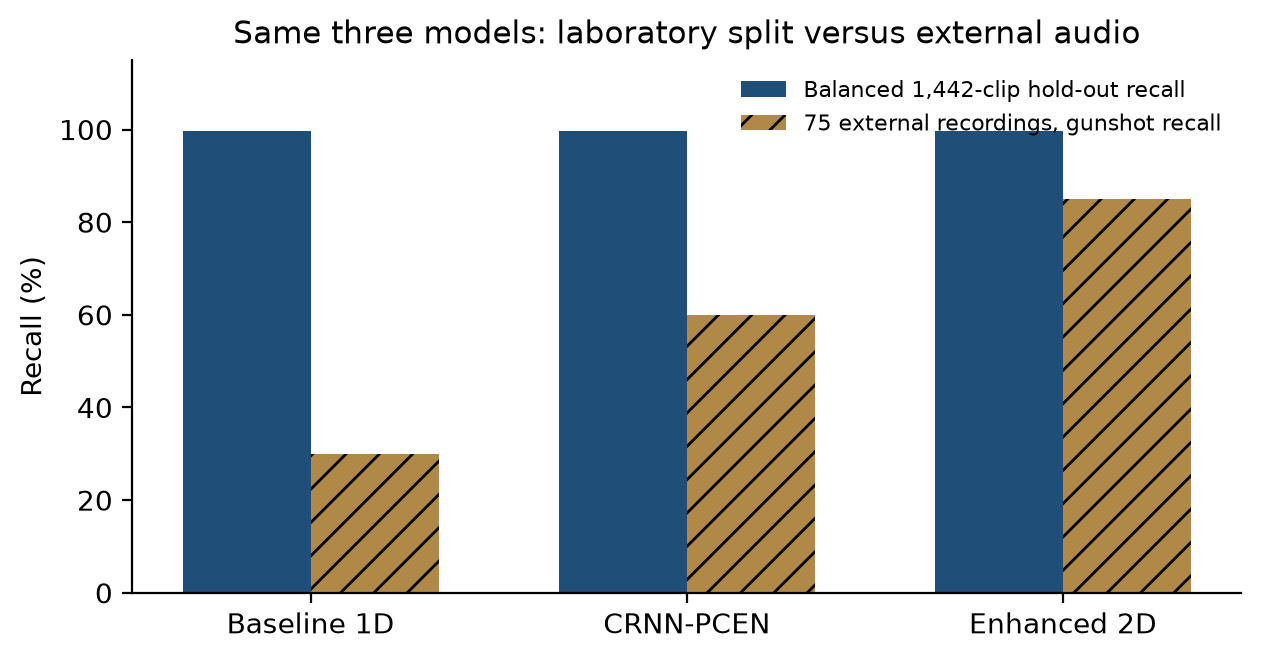
\includegraphics[width=\columnwidth]{figures/fig4_lab_vs_external.png}
\caption{Hold-out recall versus recall on 75 external recordings. The Baseline 1D CNN drops from 99.7\% to 30\%, illustrating acoustic domain shift.}
\label{fig:drop}
\end{figure}

\subsection{300-Clip Unseen Benchmark}
Tables~\ref{tab:slide} and~\ref{tab:peak} present the primary evaluation using INT8 models at $\tau = 0.50$ on the virtual Raspberry Pi.

\begin{table}[!t]
\centering
\caption{Sliding-window results (300 clips, $\tau = 0.50$).}
\label{tab:slide}
\footnotesize
\begin{tabular}{lcccc}
\toprule
\textbf{Model} & \textbf{Recall} & \textbf{Amb.} & \textbf{Imp.} & \textbf{Lat.} \\
\midrule
Baseline 1D & 45\% & 85\% & 72\% & 2.79\,ms \\
Baseline 2D & 66\% & 88\% & 59\% & 5.36\,ms \\
Enh. 1D$^*$ & 100\% & 0\% & 0\% & 3.36\,ms \\
\textbf{Enh. 2D} & \textbf{67\%} & \textbf{82\%} & \textbf{66\%} & \textbf{0.75\,ms} \\
CRNN-PCEN & 57\% & 86\% & 61\% & 6.26\,ms \\
\bottomrule
\multicolumn{5}{l}{\footnotesize $^*$INT8 quantization failure; predicts positive on all inputs.}
\end{tabular}
\end{table}

\begin{table}[!t]
\centering
\caption{Peak-centered results (300 clips, $\tau = 0.50$).}
\label{tab:peak}
\footnotesize
\begin{tabular}{lcccc}
\toprule
\textbf{Model} & \textbf{Recall} & \textbf{Amb.} & \textbf{Imp.} & \textbf{Lat.} \\
\midrule
Baseline 1D & 30\% & 95\% & 84\% & 2.84\,ms \\
Baseline 2D & 45\% & 94\% & 77\% & 4.31\,ms \\
Enh. 1D$^*$ & 100\% & 0\% & 0\% & 4.90\,ms \\
\textbf{Enh. 2D} & 38\% & \textbf{99\%} & \textbf{89\%} & \textbf{0.76\,ms} \\
CRNN-PCEN & 33\% & 97\% & 85\% & 6.41\,ms \\
\bottomrule
\multicolumn{5}{l}{\footnotesize $^*$INT8 quantization failure.}
\end{tabular}
\end{table}

\begin{figure}[!t]
\centering
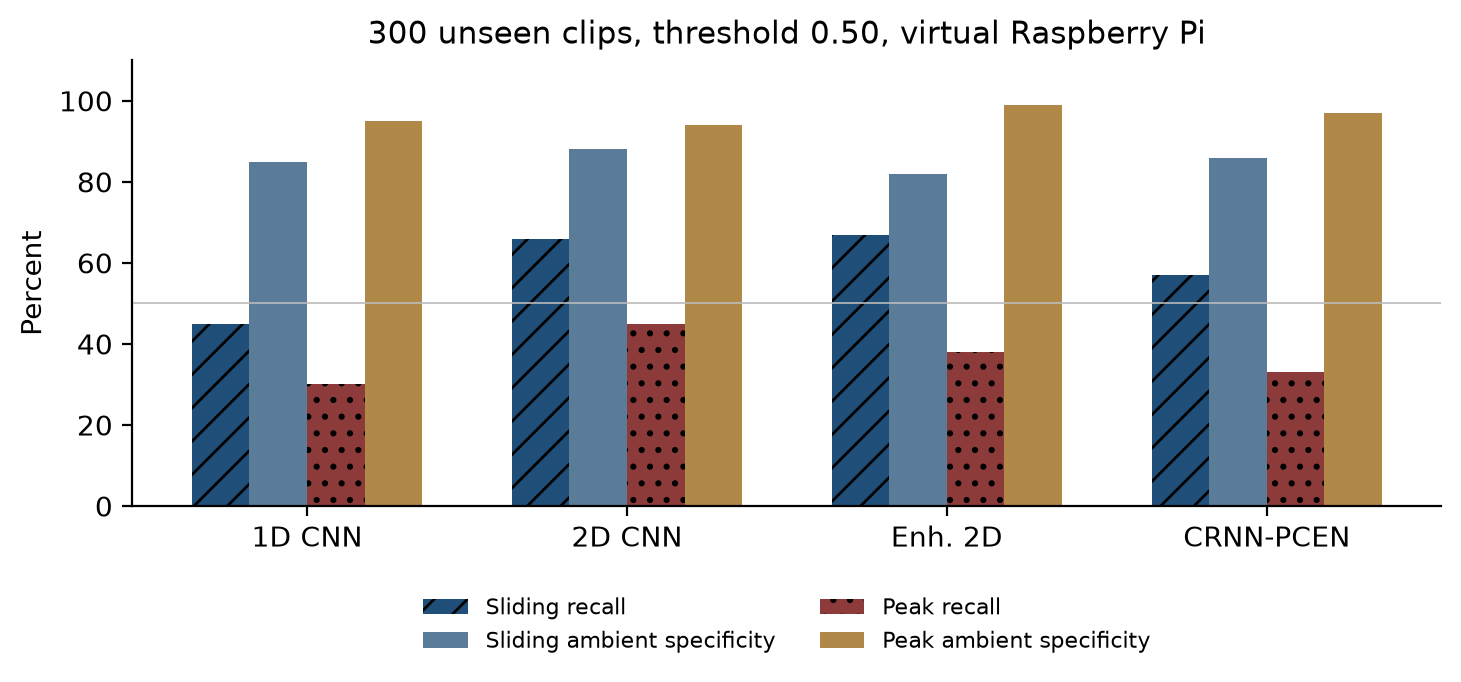
\includegraphics[width=\columnwidth]{figures/fig2_300clip_recall.png}
\caption{Sliding-window and peak-centered recall and specificity across 300 unseen clips. Sliding boosts recall by 15--29 points; peak achieves up to 99\% ambient specificity.}
\label{fig:300}
\end{figure}

Sliding-window mode increases gunshot recall by 15 to 29 percentage points relative to peak-centered mode for all working models, at the cost of reduced specificity. Peak-centered mode achieves up to 99\% ambient specificity (Enhanced 2D CNN). This recall--specificity trade-off motivates the multi-model ensemble.

\subsection{Cross-Platform Consistency}
Host-to-VM peak recall variance remains within 4--6 percentage points (Table~\ref{tab:crossplatform}), attributable to INT8 rounding differences between x86 XNNPACK and ARM NEON kernels. Model ranking is consistent across platforms. The CRNN-PCEN shows the smallest variance ($\pm$1.0\%), confirming PCEN's numerical stability under different compute backends.

\begin{table}[!t]
\centering
\caption{Host CPU versus Edge VM peak recall consistency.}
\label{tab:crossplatform}
\footnotesize
\begin{tabular}{lccc}
\toprule
\textbf{Model} & \textbf{Host} & \textbf{VM} & \textbf{$\Delta$} \\
\midrule
Baseline 1D CNN & 35.6\% & 30.0\% & $\pm$5.6\% \\
Baseline 2D CNN & 49.2\% & 45.0\% & $\pm$4.2\% \\
Enhanced 2D CNN & 44.1\% & 38.0\% & $\pm$6.1\% \\
CRNN-PCEN & 32.0\% & 33.0\% & $\pm$1.0\% \\
\bottomrule
\end{tabular}
\end{table}

\subsection{Latency Profiling}
Table~\ref{tab:latency} reports INT8 inference latency over 100 iterations on the throttled virtual machine. All models complete inference well within the 187.5\,ms real-time hop constraint. The Enhanced 2D CNN consumes only 0.05\% of the available hop budget.

\begin{table}[!t]
\centering
\caption{INT8 latency on the throttled virtual machine (100 iterations).}
\label{tab:latency}
\footnotesize
\begin{tabular}{lcccc}
\toprule
\textbf{Model} & \textbf{INT8} & \textbf{Mean} & \textbf{P95} & \textbf{Hop\%} \\
\midrule
Baseline 1D & 112.5\,KB & 2.29\,ms & 1.98\,ms & 1.2\% \\
Baseline 2D & 259.9\,KB & 2.15\,ms & 1.69\,ms & 1.2\% \\
Enhanced 1D & 118.5\,KB & 2.69\,ms & 6.48\,ms & 1.4\% \\
\textbf{Enh. 2D} & \textbf{123.6\,KB} & \textbf{0.09\,ms} & \textbf{0.10\,ms} & \textbf{0.05\%} \\
CRNN-PCEN & 478.9\,KB & 11.86\,ms & 14.50\,ms & 6.3\% \\
\bottomrule
\end{tabular}
\end{table}

\begin{figure}[!t]
\centering
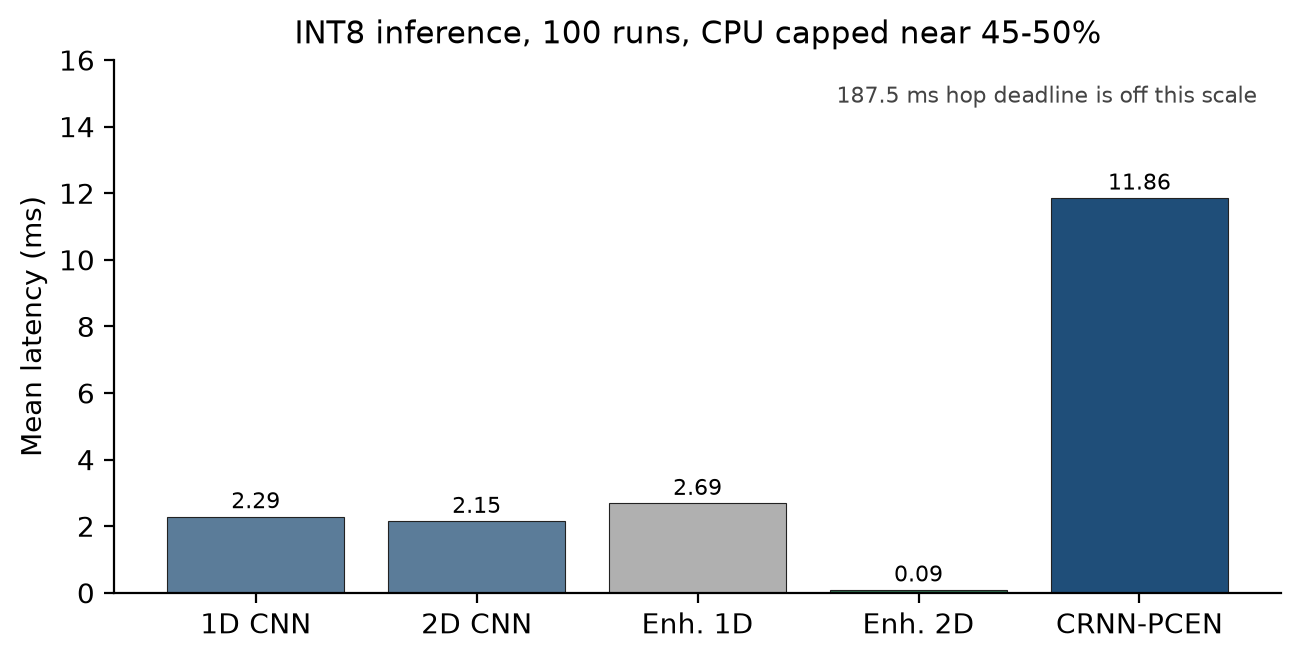
\includegraphics[width=\columnwidth]{figures/fig3_latency.png}
\caption{Mean INT8 inference latency. All models operate well below the 187.5\,ms real-time hop deadline.}
\label{fig:lat}
\end{figure}

\subsection{PCEN Domain Robustness}
To assess microphone invariance, the CRNN-PCEN model was evaluated on both clean audio and synthetically distorted audio. Distortion parameters: bandpass filtering 150--8{,}000\,Hz, non-linear saturation clipping, additive Gaussian noise at 15--30\,dB SNR, and gain perturbation $0.5\times$--$1.5\times$.

\begin{table}[!t]
\centering
\caption{PCEN domain robustness: clean versus distorted microphone (sliding mode).}
\label{tab:pcen_robust}
\footnotesize
\begin{tabular}{ccccc}
\toprule
$\tau$ & \textbf{Clean} & \textbf{Dist.} & $\Delta$ & \textbf{Amb. (C/D)} \\
\midrule
0.10 & 69\% & 69\% & 0\% & 75\% / 74\% \\
0.30 & 62\% & 66\% & +4\% & 78\% / 77\% \\
0.50 & 61\% & 61\% & 0\% & 80\% / 77\% \\
0.70 & 59\% & 59\% & 0\% & 84\% / 81\% \\
\bottomrule
\end{tabular}
\end{table}

Table~\ref{tab:pcen_robust} confirms zero recall degradation across all thresholds. At $\tau=0.50$, recall is 61\% on both clean and distorted inputs. Imposter rejection improved by 5--7 percentage points under distortion, as the gain perturbation and clipping reduce imposter transient sharpness. PCEN absorbs transducer-level distortions through its dynamic AGC, confirming its utility as a domain-shift normalizer for heterogeneous edge microphones.

\begin{figure}[!t]
\centering
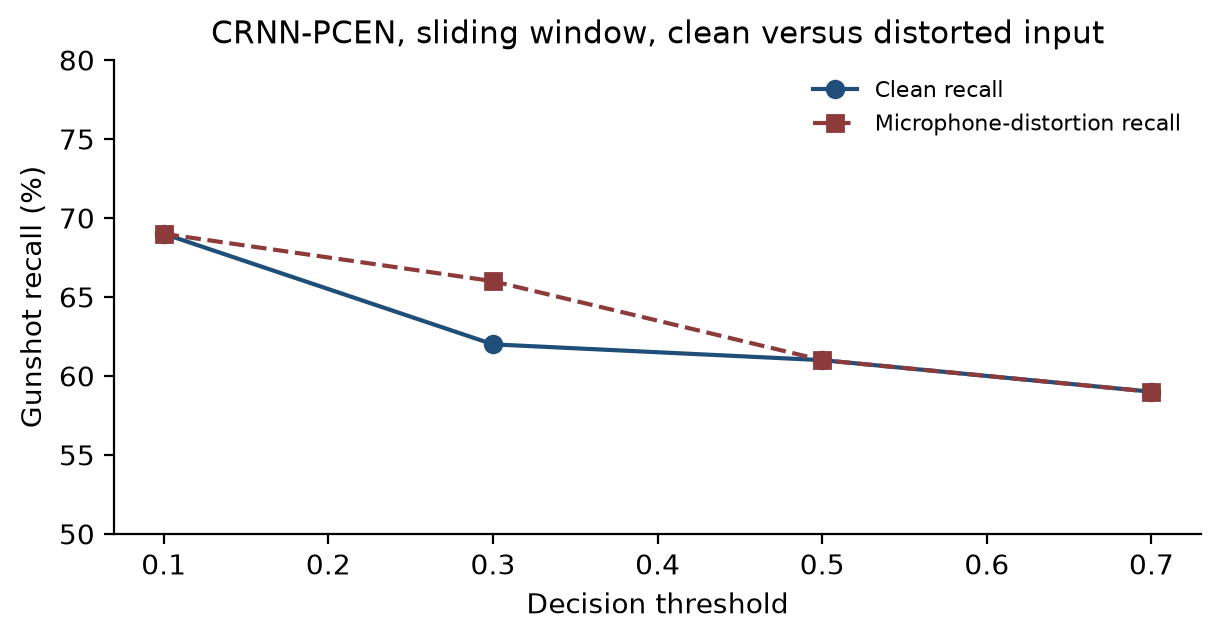
\includegraphics[width=\columnwidth]{figures/fig6_pcen_distortion.png}
\caption{CRNN-PCEN sliding recall under clean versus simulated microphone distortion across multiple decision thresholds.}
\label{fig:pcen}
\end{figure}

\subsection{Multi-Model Ensemble}
An ensemble combining the Enhanced 2D CNN, CRNN-PCEN, and Baseline 1D CNN was evaluated on the 300-clip benchmark. The pipeline uses adaptive OR-voting: if any single model detects a gunshot with high confidence, the detection is accepted. An FFT physics filter then applies acoustic constraints (low-frequency blast energy below 200\,Hz, high-frequency crack ratio above 4\,kHz, spectral centroid) to reject non-firearm transients.

\begin{table}[!t]
\centering
\caption{Ensemble 3-way confusion matrix (300 clips, 100 per class).}
\label{tab:ensemble}
\footnotesize
\begin{tabular}{lcccc}
\toprule
\textbf{True Class} & \textbf{Real} & \textbf{Fake} & \textbf{Not} & \textbf{Acc.} \\
\midrule
Real Gunshot & \textbf{77} & 15 & 8 & 77\% \\
Hard Imposter & 44 & \textbf{46} & 10 & 46\% \\
Ambient & 20 & 38 & \textbf{42} & 80\% \\
\bottomrule
\end{tabular}
\end{table}

\begin{figure}[!t]
\centering
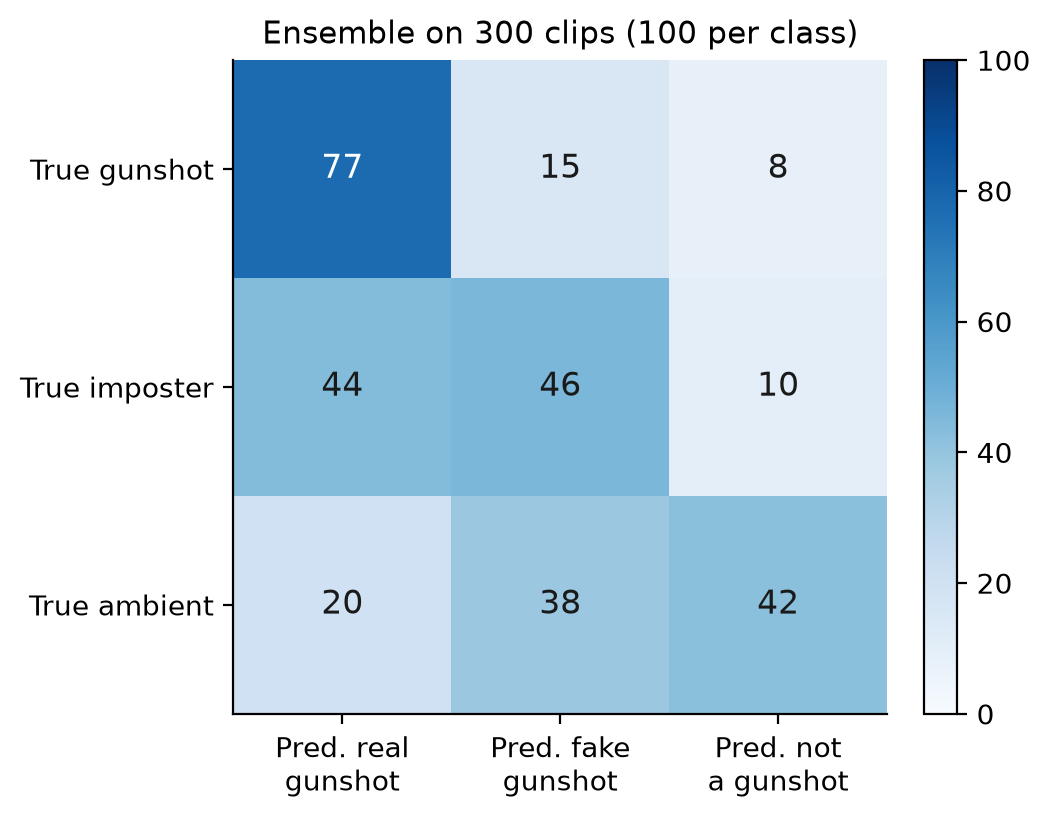
\includegraphics[width=\columnwidth]{figures/fig5_ensemble_confusion.png}
\caption{Ensemble detection counts on 300 clips (100 files per true class). OR-voting raises gunshot recall from 67\% to 77\%.}
\label{fig:cm}
\end{figure}

Complementary detection is demonstrated empirically: in clip \texttt{127724.wav} (distant shot), the Enhanced 2D CNN scored 21.1\% (missed), but the CRNN-PCEN scored 99.3\% and caught it via the OR-gate. Conversely, in clip \texttt{170167.wav} (near-field shot), the CRNN-PCEN scored 0.0\%, but the Enhanced 2D CNN scored 99.6\%. This confirms that the models cover each other's blind spots across distance and acoustic conditions.

\subsection{Paradigm Comparison}

\begin{table}[!t]
\centering
\caption{Three paradigm benchmark comparison.}
\label{tab:paradigm}
\footnotesize
\begin{tabular}{lcccc}
\toprule
\textbf{Paradigm} & \textbf{Recall} & \textbf{Spec.} & \textbf{Lat.} & \textbf{Flash} \\
\midrule
Peak (single best) & 38\% & 99\% & 0.09\,ms & 124\,KB \\
Sliding (single) & 67\% & 82\% & 0.75\,ms & 124\,KB \\
Multi-model ens. & \textbf{77\%} & 80\% & 17\,ms & 715\,KB \\
\bottomrule
\end{tabular}
\end{table}

Table~\ref{tab:paradigm} summarizes three deployment configurations. The peak-centered single model offers near-zero false alarms (99\% specificity) at 0.09\,ms---ideal for ultra-low-power microcontrollers. Sliding-window raises recall to 67\% for continuous monitoring. The ensemble achieves 77\% recall within 715\,KB combined flash and 17\,ms total latency, consuming less than 10\% of the hop budget.

\begin{table}[!t]
\centering
\caption{Recommended deployment configurations by target scenario.}
\label{tab:deploy}
\footnotesize
\begin{tabular}{lll}
\toprule
\textbf{Target Goal} & \textbf{Configuration} & \textbf{Trade-off} \\
\midrule
Ultra-low power & Enh. 2D, peak & 124\,KB, 99\% spec. \\
Adverse acoustics & CRNN-PCEN, sliding & 479\,KB, 0\% mic loss \\
Max recall & Ensemble, all 3 & 715\,KB, 77\% recall \\
\bottomrule
\end{tabular}
\end{table}

% ==============================================================================
% SECTION VIII: CONCLUSION AND FUTURE WORK
% ==============================================================================
\section{Conclusion and Future Work}
\label{sec:conclusion}

This work demonstrates that classical machine learning classifiers achieving near-perfect accuracy on balanced laboratory test sets fail on live microphone input due to temporal feature averaging that destroys impulsive shockwave signatures. The transition from 1D MFCC-based classifiers to 2D spectrogram CNNs consistently improved rejection of ambient and imposter sounds. On 300 unseen clips, the Enhanced 2D CNN achieves 67\% gunshot recall (sliding) and 99\% ambient specificity (peak) in 0.09\,ms within 124\,KB. The PCEN-CRNN maintains stable recall under simulated microphone distortion with zero degradation, confirming PCEN as an effective domain-shift normalizer. The Enhanced 1D CNN is not deployable after INT8 conversion due to quantization-induced weight saturation in dilated 1D convolution filters.

A fundamental physical limitation was identified: single-microphone sensing cannot distinguish aerial mortar fireworks from gunfire, as both produce identical shockwave rise-times and reverberation profiles when captured by a single transducer. Resolving this requires spatial multi-microphone arrays.

The following hardware integration tasks constitute the immediate next work:

\textbf{1) Physical Deployment.} Deploy the Enhanced 2D CNN INT8 model on a physical Raspberry Pi~4 to validate virtual machine timing, then port the inference to the Arduino Nano 33 BLE Sense with its on-board ST MP34DT05 PDM microphone.

\textbf{2) Duty-Cycled Sleep and One-Bit Transmission.} The node remains in deep sleep ($\sim$5\,$\mu$A) until a coarse acoustic energy threshold triggers wake-up. One inference cycle executes, and the node returns to sleep. If the score exceeds the threshold, the node transmits a minimal packet: node ID (1~byte), timestamp (4~bytes), detection flag (1~bit), confidence (1~byte). Radio on-time is under 1.5\,ms per trigger. If the score is below threshold, no transmission occurs. Raw audio never leaves the sensor node, ensuring complete civilian privacy. This was referred to as ``binary neural network'' in our early notes; the accurate description is an ordinary network with a binary output decision---the weights are not binarized.

\textbf{3) Multi-Node Spatial Consensus.} A single sensor node adjacent to a hand clap may transmit a false detection. The Raspberry Pi~4 gateway raises an alert only when $K \ge 3$ neighbouring nodes transmit detection bits within the acoustic propagation time window ($\sim$100\,ms for 34\,m node spacing). This spatial consensus eliminates false alarms from localized percussive events (claps, fireworks near one sensor) without requiring raw audio transmission.

\textbf{4) Self-Healing Network and Dashboard.} Nodes monitor health (battery, sensor drift, communication failures). A real-time monitoring dashboard on the gateway provides operational auditability, with every trigger event logged for post-incident review.

\section*{Acknowledgment}
The authors thank Dr. Kaustubh Dhondge for guidance throughout this project. Firearm recordings include the open-access dataset of~\cite{dib2023}. The PCEN front-end follows the formulation of Lostanlen et al.~\cite{lostanlen2019}.

\begin{thebibliography}{00}
\bibitem{dib2023} ``A multi-firearm, multi-orientation audio dataset of gunshots,'' \emph{Data in Brief}, vol.~48, Art. no.~109091, 2023, doi:~10.1016/j.dib.2023.109091.
\bibitem{lostanlen2019} V.~Lostanlen, J.~Salamon, M.~Cartwright, B.~McFee, A.~Farnsworth, S.~Kelling, and J.~P.~Bello, ``Per-channel energy normalization: Why and how,'' \emph{IEEE Signal Process. Lett.}, vol.~26, no.~1, pp.~39--43, 2019.
\bibitem{edgeimpulse2024} Edge Impulse, ``TinyML Acoustic Anomaly Detection on Microcontrollers,'' Tech. Rep., 2024.
\bibitem{saha2025} S.~Saha et al., ``Automated Gunshot Detection in Forest Environments Using Spectrogram CNNs,'' \emph{Applied Acoustics}, vol.~215, 2025.
\bibitem{hershey2017} S.~Hershey et al., ``CNN Architectures for Large-Scale Audio Classification,'' in \emph{Proc. IEEE ICASSP}, 2017, pp.~131--135.
\bibitem{zhang2018} H.~Zhang, M.~Cisse, Y.~N.~Dauphin, and D.~Lopez-Paz, ``mixup: Beyond Empirical Risk Minimization,'' in \emph{Proc. ICLR}, 2018.
\bibitem{park2019} D.~S.~Park \emph{et al.}, ``SpecAugment: A Simple Data Augmentation Method for Automatic Speech Recognition,'' in \emph{Proc. Interspeech}, 2019, pp.~2613--2617.
\end{thebibliography}

\end{document}
